The first 32-bit word of the header is interpreted as the message length in bytes, little-endian. The next 8-bit byte is the opcode of the message, followed by 3 padding bytes.
If the end of the file is encountered while reading a message header, or while reading
the header-specified length of the message payload, an error will be reported and the
component will terminate.  The following Messaging File Field Layout shows the layout of a file: 

\begin{figure}[ht]
	\centerline{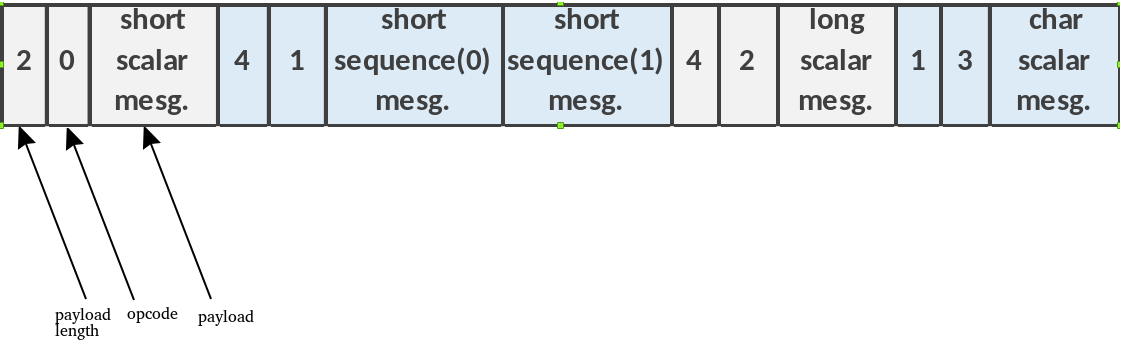
\includegraphics[scale=0.45]{MessageMode}}
	\caption{Messaging File Field Layout}
\end{figure}